\fancyfoot[C]{Sandri}
\section{Laserschneiden}
	Beim Laserschneiden k�nnen meist flache Werkstoffe verschiedenster Dicke mithilfe von einem konzentrierten Laserstrahl ohne Ber�hrung geschnitten werden. Der Laserstrahl erhitzt dabei das Material an einem Punkt so stark, dass es sofort schmilzt oder verdampft. Mithilfe von einem Schneidgas kann das nun geschmolzene Material aus der Schnittfuge geblasen werden. Mit dieser Technik k�nnen eine Vielzahl an Materialien, wie zum Beispiel Holz, Acryl, Schaumstoff oder auch diverse Metalle wie Stahl, Edelstahl und Aluminium geschnitten werden. \cite{Trumpf2024}
	
	\subsection{Arten von Lasern}
	Test
	
	\subsection{Schneiden verschiedener Werkstoffe}
	Test
	
	\subsection{Sicherheitsvorkehrungen}
	Die Strahlung von Lasern kann sehr schnell f�r Auge und Haut gef�hrlich werden, deswegen gibt es einige wichtige Sicherheitsvorkehrungen, die eingehalten werden m�ssen.
	\begin{itemize}
		\item Laserstrahl nie auf andere Personen richten
		\item Laserstrahl nie auf direkt reflektierende Oberfl�chen richten
		\item Nicht in den direkten oder reflektierten Strahl blicken
		\item Keine optischen Instrumente(z.B. Lupe oder Fernglas) zur Beobachtung des Laserstrahl verwenden
		\item Niemals die Laserquelle manipulieren.
	\end{itemize}
	Laserger�te werden au�erdem vom Hersteller gem�� ihrem Gef�hrdungspotenzial in verschiedene Klassen eingeteilt. Ma�geblich daf�r ist die DIN-Norm EN 60825-1. Die Klassen sind so eingeteilt, dass mit zunehmender Gefahr die Klassen h�her wird. Diese Klassen reichen von 1 bis 4 und sind in 1, 1M, 1C, 2, 2M, 3A, 3R, 3B und 4 aufgeteilt.\cite{Strahlenschutz2024}
	
	\begin{figure}[H]
		\centering
		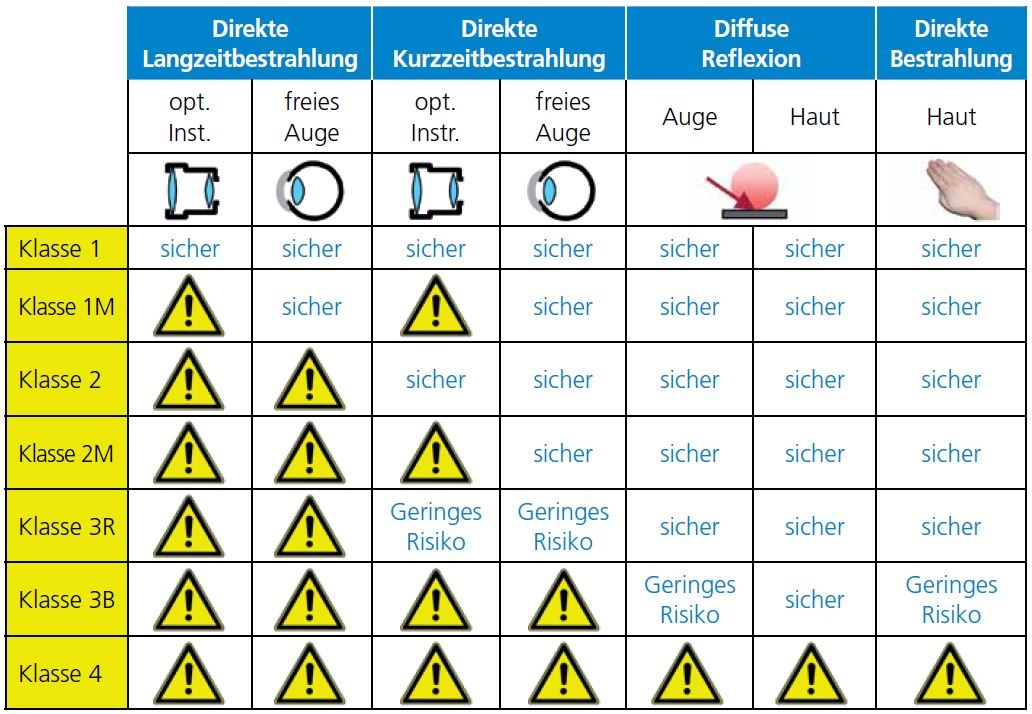
\includegraphics[scale=0.5]{./3_Stand_der_Technik/Abbildungen/Laserklassen_1}
		\caption{Laser Sicherheitsklassen\cite{eval.at2024a}}
	\end{figure}